%TO DO
%Überleitung zu 3.1 und 3.2
%Etwas mehr QML einfließen lassen -> klarer roter Faden

\section{Quantum Machine Learning in der NISQ-Ära}
\label{sec:nisq}

In den letzten zwei Dekaden war ein explosives Wachstum sowohl in der Theorie als auch in der Praxis des Quantum Computings zu verzeichnen \cite{quantummethodssupervised1}. Ein großer Begriff ist hierbei die Quantum Supremacy – also die Quantenüberlegenheit. Sobald diese erreicht ist, lassen sich viele Probleme auf einem Quanten Computer um ein Vielfaches effizienter lösen als auf den leistungsstärksten Supercomputern. Laut IBM ist dieser Zustand ab etwa 1000 Qubits denkbar. Die Roadmap des amerikanischen IT-Unternehmens – stolz auf Ihre bisherige Arbeit mit dem 5-Qubit Quantum Canary Prozessor und dem dem 27-Qubit Quantum Falcon Prozessor – bringt 2020 den 65-Qubit Quantum Hummingbird Prozessor auf den Markt und legt Pläne für den 2021 erscheinenden 127-Qubit Quantum Eagle Prozessor offen. Große Möglichkeiten bieten sich schon durch diese technologischen Sprünge, doch man ist noch weit entfernt von den angesprochenen 1000 Qubits, auch wenn IBM 2022 den 433-Qubit Prozessor Quantum Osprey und für 2023 den 1,121-Qubit Quantum Condor Prozessor angekündigt hat \cite{roadmapIBM}.  \\


Doch auch schon mit 50-100 Qubits ist es Quantum Computern möglich, die Fähigkeiten klassischer Computer zu übertreffen. Ein Problem hierbei stellt allerdings das Rauschen der Quantum Gates dar, durch dieses wird die Anzahl der verlässlich eingesetzten Quanten Schaltkreise limitiert  \cite{preskill2018quantum}.\\

In der Praxis lassen sich verlässliche Quanten Computer also bisher nur mit einer geringen Menge an Qubits herstellen. \\
Wir befinden uns aktuell in der Phase der Entwicklung von Quantencomputertechnologie die J. Preskill mit „Noisy Intermediate Scale Quantum“, kurz NISQ, betitelte. Gemeint sind damit rauschanfällige Systeme mit maximal fünfzig bis hundert Qubit \cite{preskill2018quantum}.  Der Begriff wurde weitgehend übernommen, wobei manche Autoren die Obergrenze bis tausend Qubit setzen. Somit stellt diese Technologie einen Zwischenschritt zwischen klassischem Machine Learning und dem reinen Quantum Machine Learning dar.

Auch wenn Quanten Computer aktuell noch zu klein sind, um Machine Learning Algorithmen zu implementieren, wurde in Simulationen auf klassischen Computern gezeigt dass Quanten Supervised Learning voraussichtlich noch in der NISQ-Ära möglich sein wird \cite{chen2020variational}.\\ 


\subsection{Hürden der NISQ Technologie}
Im Folgenden soll nun betrachtet werden, welche Schwierigkeiten sich aus der geringen Anzahl an Qubits in NISQ Prozessoren ergeben. \\

Das „Noisy“ in NISQ bezieht sich vor allem auf das maschineninterne Rauschen, das die Gates und Qubits selbst abgeben und welches den Zustand umliegender Qubits beeinflussen kann. Je länger eine Berechnung nun läuft, desto größer wird der Einfluss des Rauschens und desto wahrscheinlicher wird es, dass der Status der Qubits verfälscht wird \cite{murali2019noise}. \\

Hinzu kommt, dass Methoden zur Fehlerkorrektur in NISQ Computern nicht effizient möglich sind, da sie die Kapazität der für die eigentliche Berechnung nutzbaren Qubits zu sehr einschränkt. Nach Shor's Algorithmus werden für jedes Berechnungs-Qubit neun Qubits zur Korrektur benötigt.
\\
Hieraus folgt, dass die Kohärenz-Zeit in NISQ Computern relativ gering ist. Nach Ablauf dieser Dauer sind ausgelesene Ergebnisse nicht mehr verlässlich. 
In den Benchmarks zum IBM Q System One wurde beispielsweise eine durchschnittliche Kohärenzzeit von 73\textmu s angegeben \cite{benchmarksIBM}.


\subsection{Hybride Methoden}
Aufgrund dieser Hürden in der Menge nutzbarer Qubits und in der Kontrolle selbiger über längere Zeiträume wird reines Quantum Machine Learning voraussichtlich innerhalb der NISQ-Ära nicht umsetzbar sein.\\
Eine Zwischenlösung könnten Hybride Methoden für Quantum Assisted Machine Learning (QAML) liefern, bei denen klassische und Quanten Computer gemeinsam eingesetzt werden.


\label{subsec:hybrid}
\subsubsection{Motivation}

Die kurzfristige Implementierung von QAML Algorithmen, die mit dem letzten Stand der Technik von klassischen Machine Learning Algorithmen mithalten können, wird höchstwahrscheinlich nicht durch eine reine Adaption der bekannten ML Algorithmen erreicht. Durch die Limitationen der nicht störfreien Quanten Gatter und der dadurch limitierten Anzahl an fehlerfrei verwendbaren Qubits kommt die Idee auf, klassisches Maschinelles Lernen mit Quantum Machine Learning zu kombinieren, d.h. ein Hybrid aufzubauen, das besser als Quantum Assisted Machine Learning zu bezeichnen ist. Idee dahinter ist es nun, ein klassisches neuronales Netz aufzubauen und rechentechnisch schwierige Unterschritte auf einen Quantencomputer auszulagern \cite{opportunitieschallenges1}. \\
Die Herangehensweise: Folgende theoretische Zeichnung soll nun in die Tat umgesetzt und mithilfe von klassischen und Quanten Computern implementiert werden.\\


\begin{figure}[h]
\floatbox[{\capbeside\thisfloatsetup{capbesideposition={right},capbesidewidth=4cm}}]{figure}[\FBwidth]
{\caption{Theoretischer, abstrakter Aufbau eines Quantum Machine Learning Hybrids. \cite{opportunitieschallenges1}}\label{fig:test}}
{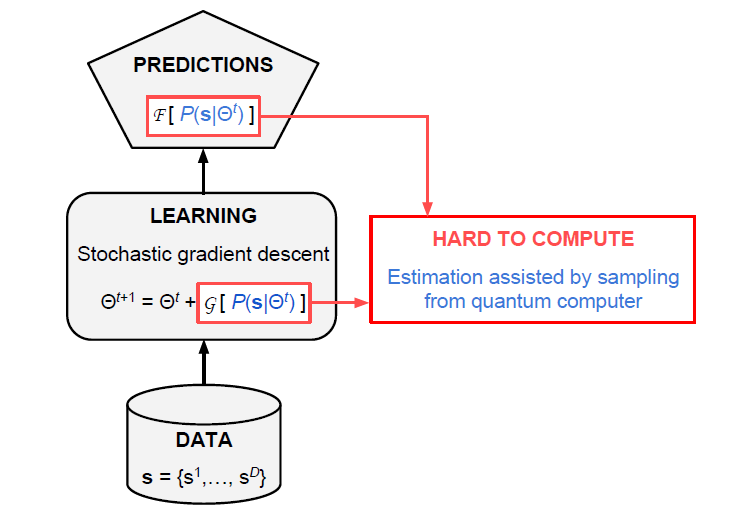
\includegraphics[width=10cm]{QML/images/3-2-1.PNG}}
\end{figure}\\


\subsubsection{Herangehensweise}

Um die begrenzten Kapazitäten von NISQ Computern ideal für Machine Learning nutzen zu können, liegt es nahe, Hybride aus Quanten- und klassischen Computern zu benutzen. Mit klassischen Computern als Steuer- bzw. Kontrolleinheit und zur Aufbereitung von Ein- und Ausgabedaten, könnte die gesamte Rechenleistung und -dauer der Quanten Computer für aufwändige ML-Algorithmen genutzt werden \cite{wittek2014quantum}.\\


Eine grundlegende Komponente in dem Hybriden Ansatz des Machine Learning ist der Informationsfluß zwischen klassischem Computer und seinem Quantum Konterpart. Jedoch stellt gerade diese essentielle Grundlage schon eine große Herausforderung dar (Eingabe- /Ausgabeproblem). Diese Schwierigkeiten wurden festgestellt bei dem Versuch, Restricted Boltzmann Maschinen (RBMs) oder auch Deep Belief Networks (DBNs) mit Quanten Geräten zu unterstützen \cite{opportunitieschallenges5}. \\

 Schafft man es jedoch, diese Hürde - neben weiteren anderen -  zu überwinden, so ist es möglich, den Lernprozess initial auf einem klassischen Computer laufen zu lassen. Dies gilt da die Model Parameter unter dem "Noise"-Level und der Präzision des Quanten Geräts liegen können. Bei Bedarf kann dann der Quanten Computer angewiesen werden, die Aufgabe zu übernehmen \cite{opportunitieschallenges5}. \\


\begin{figure}
\floatbox[{\capbeside\thisfloatsetup{capbesideposition={right},capbesidewidth=3cm}}]{figure}[\FBwidth]
{\caption{Funktionsweise eines Quantum Machine Learning Hybrids am Beispiel von Zahlenerkennung. \cite{opportunitieschallenges1}}\label{fig:test}}
{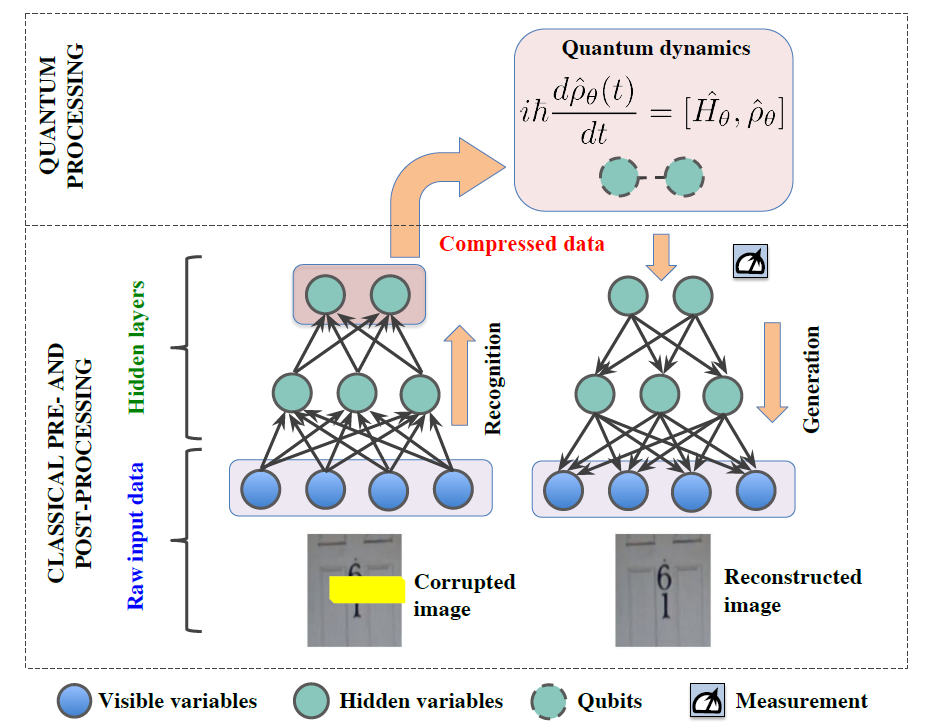
\includegraphics[width=13cm]{QML/images/3-2-2.PNG}}
\end{figure}


 Da aber mit wachsender Datenmenge die Bearbeitungsdauer von In- und Output steigt \cite{biamonte2017quantum}, wird vermutlich mit Ende der NISQ-Ära eine andere Methode hierfür gefunden werden müssen. Beim NISQ Machine Learning sind die Datenmengen aufgrund der verfügbaren Rechenkapazität der Quantencomputer allerdings sowieso sehr begrenzt, somit sollte sich diese Methode für Near-Term-Anwendungen dennoch gut eignen.\\

